\ifdefined\ishandout
\documentclass[handout]{beamer}
\else
\documentclass{beamer}
\fi

\usepackage[frenchb]{babel}
\usepackage[T1]{fontenc}
\usepackage[latin1]{inputenc}
\usepackage{hyperref}
\usepackage{multirow}
\usepackage{listings}
\usepackage{fancyvrb}
\usepackage{tikz}
\usepackage{framed}
\usepackage{algorithm}
\usepackage{algorithmic}
\usepackage{xcolor}
\usepackage{color, colortbl}
\usepackage{handoutWithNotes}
\usepackage{amsmath}
\usetikzlibrary{shapes.geometric}
\usetikzlibrary{positioning}
\usetikzlibrary{shapes.arrows, chains}
\usetikzlibrary{arrows,calc}
\usetikzlibrary{shapes.multipart}
\usepackage{array}
\usetheme{Boadilla}
\definecolor{BlueGreen}{cmyk}{0.85,0,0.33,0}
\definecolor{Gray}{rgb}{0.8,0.8,0.8}

\ifdefined\ishandout
\pgfpagesuselayout{3 on 1 with notes}[a4paper,border shrink=5mm]
\usecolortheme{dove}
\else
\usecolortheme{dolphin}
\fi


\lstnewenvironment{codeC}
{ \lstset{language=C,
    otherkeywords={printf,scanf}}
}
{}

\ifdefined\ishandout
\definecolor{mygreen}{rgb}{0,0,0}
\definecolor{mymauve}{rgb}{0,0,0}
\definecolor{myblue}{rgb}{0,0,0}
\else
\definecolor{mygreen}{rgb}{0,0.6,0}
\definecolor{mymauve}{rgb}{0.58,0,0.82}
\definecolor{myblue}{rgb}{0,0,1}

\fi

\definecolor{mygray}{rgb}{0.5,0.5,0.5}


\lstset{language=C,
% breakatwhitespace=false,         % sets if automatic breaks should only happen at whitespace
%  breaklines=true,                 % sets automatic line breaking
%  captionpos=b,                
commentstyle=\itshape\color{mymauve},
keywordstyle=\bfseries\color{myblue},
%numbers=left,                    % where to put the line-numbers; possible values are (none, left, right)
%  numbersep=8pt,                   % how far the line-numbers are from the code
%  numberstyle=\tiny\color{mygray}, % the style that is used for the line-numbers
  rulecolor=\color{black},         % if not set, the frame-color may be changed on line-breaks within not-black text (e.g. comments (green here))
%  showspaces=false,                % show spaces everywhere adding particular underscores; it overrides 'showstringspaces'
  showstringspaces=false,          % underline spaces within strings only
%  showtabs=false,                  % show tabs within strings adding particular underscores
%  stepnumber=2,                    % the step between two line-numbers. If it's 1, each line will be numbered
  stringstyle=\color{mygreen},     % string literal style
%  tabsize=2 
}
\ifdefined\ishandout
\newcommand{\red}{\textbf}
\else
\newcommand{\red}{\textcolor{red}}
\fi
%\newcommand \emph
%Default size : 12.8 cm * 9.6 cm

\newcommand{\tmark}[1]{\tikz[remember picture, baseline=-.5ex]{\coordinate(#1);}}

\ifdefined\ishandout
\newenvironment<>{codeblock}[1]{%begin
  \setbeamercolor{block title}{fg=black,bg=lightgray!80}%
  \begin{block}{#1}}
  % \begin{codeC}}
  %  {\end{codeC}
{  
\end{block}}

\newenvironment<>{termblock}[1]{
    \setbeamercolor{block title}{fg=black,bg=lightgray!90}%
    \begin{block}{#1}
}
%     \begin{Verbatim}}
{%\end{Verbatim}
\end{block}
}

\definecolor{bluegreen}{RGB}{0,0,0}
%\definecolor{bluegreen}{rgb}{0,0.6,0.8}
\else

\newenvironment<>{codeblock}[1]{%begin
  \setbeamercolor{block title}{fg=darkgray,bg=yellow}%
  \begin{block}{#1}}
  % \begin{codeC}}
  %  {\end{codeC}
{  
\end{block}}

\newenvironment<>{termblock}[1]{
    \setbeamercolor{block title}{fg=white,bg=lightgray}%
    \begin{block}{#1}}
%     \begin{Verbatim}}
{%\end{Verbatim}
\end{block}
}

\definecolor{bluegreen}{RGB}{0,149,182}
%\definecolor{bluegreen}{rgb}{0,0.6,0.8}
\fi

%\newcommand{\output}[1]{
\setbeamertemplate{navigation symbols}{}
\newcommand{\bvrb}{\Verb[commandchars=���,formatcom=\color{bluegreen}]}
\newcommand{\footvrb}{\footnotesize\Verb}
\newcommand{\vrbalert}[2][]{\visible<#1>{#2}}
%%% Commande pour les listes/arbres
\newcommand{\mvide}{\nodepart{one} \nodepart{two}}
\newcommand{\tvide}{\nodepart{one} \nodepart{two} \nodepart{three}}

%%Fin des commandes pour les listes/arbres.


\newcommand<>{\case}[2]{%
\filldraw (#1,#2) rectangle (1+#1,1+#2);}
%%% Param�tres du cours (� r�gler)
%Num�ro du cours
\newcommand{\nb}{3}
\title[cours n�3]{Les tableaux}
\author[]{julien.brajard@upmc.fr}
\institute[Polytech'UPMC]{Polytech'UPMC}
\date{02 Octobre 2017}
\begin{document}

\begin{frame}
\titlepage
\centering{
\url{https://moodle-sciences.upmc.fr} (cours Informatique G�n�rale MAIN-ROB)}
\end{frame}
% !TEX encoding = IsoLatin9
\section{Tableaux statiques}
\begin{frame}
  \begin{columns}
    \column{4.8cm}
    \tableofcontents[currentsection,hideothersubsections]
    \column{7cm}
    \centering{
      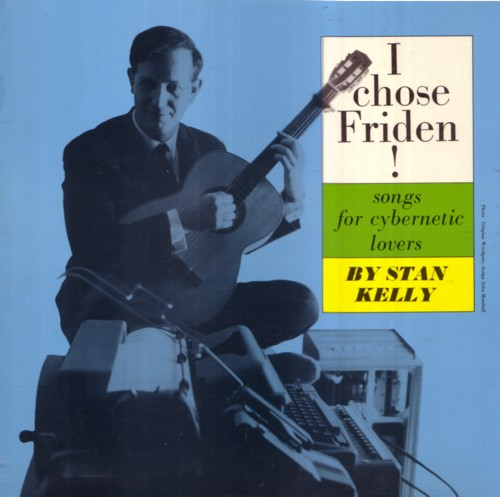
\includegraphics[width=4cm]{fig/kelly.jpg}
      
      \textit{``Should array indices start at 0 or 1 ? 
My compromise of 0.5 was rejected without, I thought, proper consideration''}\\
      \small{
        \hfill Stan Kelly-Bootle (1929-2014)\\
               \hfill informaticien, auteur-compositeur}
    }
  \end{columns}
  
\end{frame}

\begin{frame}
\frametitle{G�n�ralit�s}
\begin{itemize}
  \setlength\itemsep{1em}
\item Un tableau est un ensemble d'�l�ments de m�me type
d�sign� par un identificateur unique.\\
\item Chaque �l�ment est rep�r� par un \red{indice} pr�cisant
sa position au sein de l'ensemble.\\
\item Il se d�clare en m�me temps que les autres variables.\\
\item Il existe deux grandes familles de tableaux : \\
\begin{itemize}
\item Les tableaux unidimensionnels (vecteurs)\\
\item Les tableaux multidimensionnels (matrices)\\
\end{itemize}
\end{itemize}
\end{frame}

\begin{frame}[fragile]
\frametitle{D�claration de tableaux unidimensionnels}
\begin{itemize}
\item On doit r�server un emplacement m�moire pour un certain
nombre d'�l�ments.\\
{\centering{
\bvrb|�textit�type nom_tableau�[ �textit�nb_elements� ];|\\
}}
\begin{itemize}
\item \bvrb|�textit�type�| est le type des �lements du tableau \bvrb|�textit�nom_tableau�|\\
\item \bvrb|�textit�nb_elements�| est le nombre d'�l�ments que contient le tableau.\\
\end{itemize}

\item Conventionnellement, \red{la premi�re position porte le num�ro 0}.
Les indices vont donc de \verb|0| � \Verb|nb_elements-1|
\end{itemize}
\begin{codeblock}{}
%\vspace{-.3cm}
\lstset{escapeinside={��}}
%\lstset{basicstyle=\scriptsize}
\begin{codeC}
int tab[10] ; // tab est un tableau de 10 entiers
float zz[5] ; // zz est un tableau de 5 r�els
char y[12] ; // y est un tableau de 12 caract�res
\end{codeC}
\end{codeblock}
\end{frame}

\begin{frame}
\frametitle{Quelques r�gles}
\begin{itemize}
 \setlength\itemsep{1em}
\item Chaque �l�ment est stock� dans une case d'un tableau
(localis� par un \red{indice}).\\
\item Un �l�ment de tableau est une variable :
\begin{itemize}
\item On peut l'initialiser.\\
\item On peut l'utiliser dans une expresssion.\\
\end{itemize}
\item Le premier �l�ment du tableau est � l'indice \red{0}.\\
\item La dimension d'un tableau (nombre d'�l�ments) ne peut �tre
qu'une constante ou une expression constante (pas une variable).\\
\item Il faut faire tr�s attention aux probl�mes de d�bordement d'indice
(cas o� l'on veut acc�der � un indice de tableau sup�rieur au nombre
d'�l�ments pr�vus).\\
\end{itemize}

\end{frame}

\begin{frame}[fragile]
\frametitle{Initialisation des �l�ments (1)}

\begin{itemize}
\item Initialisation de l'�lement d'indice \verb|k| :\\

\begin{columns}
\column{0.5\textwidth}
\begin{block}{}
\bvrb|�textit�nom_tableau�[k] = �textit�valeur� ;|\\
\bvrb|�textit�nom_tableau�[k] = �textit�expression� ;|\\
\end{block}
\column{0.45\textwidth}
\begin{codeblock}{}
\vspace{-.3cm}
\lstset{escapeinside={��}}
\lstset{basicstyle=\scriptsize}
\begin{codeC}
tab[0]=5 ;
/* le premier �l�ment du 
tableau tab a pour 
valeur 5*/
\end{codeC}
\vspace{-.3cm}
\end{codeblock}
\end{columns}
\item Initialisation � la d�claration
\begin{codeblock}{}
\vspace{-.3cm}
\lstset{escapeinside={��}}
\lstset{basicstyle=\scriptsize}
\begin{codeC}
//Place les valeurs 1,2,3,4,5 dans chacun des 
//5 �l�ments du tableau :
int tab[5] = {1,2,3,4,5};

//Ne remplit que certains indices (ici 2 et 4) :
int tab[5] = {,,3,,5};

//Ne remplit que les 2 premiers indices (0 et 1) :
int tab[5] = {2,3};

//Determine automatiquement la taille du tableau (en fonction
//du nombre de valeurs :
int tab[] = {1,2,3,4,5};

\end{codeC}
\vspace{-.3cm}
\end{codeblock}
\end{itemize}

\end{frame}

\begin{frame}[fragile]
\frametitle{Initialisation des �l�ments (2)}
\begin{block}{}
Initialisation des �l�ments dans une boucle \bvrb|for|
\end{block}
\begin{columns}[t]
\column{0.45\textwidth}
\begin{table}
\centering
\begin{tabular}{|c|c|c|c|c|}
\hline
0 & 0 & 0 & 0 & 0 \\
\hline
\end{tabular}
\end{table}
\begin{codeblock}{}
\vspace{-.3cm}
\lstset{escapeinside={��}}
%\lstset{basicstyle=\scriptsize}
\begin{codeC}
int j ; //ind. de boucle
int Tab[5] ;

for (j=... ; ... ; ...) 

{

...

}

\end{codeC}
\vspace{-.3cm}
\end{codeblock}

\column{0.45\textwidth}
\begin{table}
\centering
\begin{tabular}{|c|c|c|c|c|}
\hline
0 & 2 & 4 & 6 & 8 \\
\hline
\end{tabular}
\end{table}
\begin{codeblock}{}
\vspace{-.3cm}
\lstset{escapeinside={��}}
%\lstset{basicstyle=\scriptsize}
\begin{codeC}
int j ; //ind. de boucle
int Tab[5] ;

for (j=... ; ... ; ...) 

{

...

}

\end{codeC}
\vspace{-.3cm}
\end{codeblock}

\end{columns}

\end{frame}

\begin{frame}[fragile]
\frametitle{Un exemple (version 1)}
\begin{columns}
\column{0.5\textwidth}
\begin{codeblock}{}
\vspace{-.3cm}
\lstset{escapeinside={��}}
\lstset{basicstyle=\scriptsize}
\begin{codeC}
#include <stdio.h>

/* Remplissage d'un tableau de
notes et calcul de la moyenne */

int main()
{
  float notes[50], moy=0.0;
  int i;
  
  for (i=0;i<50;i++)
  {
    printf("\Entrez la note: ");
    scanf("%f",&notes[i]);
    moy += notes[i];
  }
  printf("\nmoyenne = %f",moy/50);
}
\end{codeC}
\vspace{-.3cm}
\end{codeblock}

\column{0.5\textwidth}
\begin{itemize}
\item On remplit les 50 �l�ments du 
tableau (utilisation d'une boucle
\bvrb|for|)\\
\item \Verb|i| sert d'indice pour parcourir
les �l�ments du tableau.\\
\item La moyenne est calcul�e en ajoutant
� chaque pasasge de boucle, la nouvelle 
note saisie au clavier (\bvrb|scanf|)\\
\end{itemize}

\end{columns}

\end{frame}

\begin{frame}[fragile]
\frametitle{Probl�mes dans l'exemple}
\begin{itemize}
 \setlength\itemsep{1em}
\item Utilisation non s�curis�e de \bvrb|scanf|\\
\begin{itemize}
\item V�rification du nombre d'�l�ments correctements
entr�s
\item "Nettoyage de la m�moire tampon".\\
\end{itemize}
\item Probl�me pratique si on veut modifier la taille
du tableau.\\
\end{itemize}
\end{frame}


\begin{frame}[fragile]
\frametitle{Un exemple (version 2)}
\begin{columns}
\column{0.5\textwidth}
\begin{codeblock}{}
\vspace{-.3cm}
\lstset{escapeinside={��}}
\lstset{basicstyle=\scriptsize}
\begin{codeC}
#include <stdio.h>
#define NMAX 50

/* Remplissage d'un tableau de
notes et calcul de la moyenne */

int main()
{
  float notes[NMAX], moy=0.0;
  int i;
  
  for (i=0;i<NMAX;i++)
  {
    printf("\Entrez la note: ");
    scanf("%f",&notes[i]);
    moy += notes[i];
  }
  printf("\nmoyenne = %f",moy/NMAX);
}
\end{codeC}
\vspace{-.3cm}
\end{codeblock}

\column{0.45\textwidth}
D�finition de la taille du 
tableau par un \bvrb|#define| (fortement
conseill�).\\

\begin{alertblock}{}
Si la valeur de \Verb|NMAX| est modifi�e,
il faut recompiler.
\end{alertblock}
\end{columns}

\end{frame}

\begin{frame}[fragile]
\frametitle{Les tableaux multidimensionnels}
\begin{block}{D�claration}
\bvrb|�textit�type nom_tableau �[�textit�dim1�][�textit�dim2�]...[�textit�dimN�];|
\end{block}

\begin{codeblock}{Initialisation}
\vspace{-.3cm}
\lstset{escapeinside={��}}
\lstset{basicstyle=\scriptsize}
\begin{codeC}
//tableau vu comme 5 tableaux de deux �l�ments chacun
int tab[5][2] = {{1,2},{3,4},{5,6},{7,8},{9,10}};

//El�ments rang�s en m�moire automatiquement :
int tab[5][2] = {1,2,3,4,5,6,7,8,9,10};

//Omission de valeurs :
int tab[5][2] = {1,,3,,,,7,8,9,};

//Acc�s � un indice (apr�s d�claration):
tab[3][0] = 12 ;

\end{codeC}
\vspace{-.3cm}
\end{codeblock}

\end{frame}

\begin{frame}
\frametitle{Algorithmes classiques sur les tableaux}
\begin{itemize}
 \setlength\itemsep{1em}
\item Initialisation d'un tableau � une valeur constante.\\
\item Copie d'un tableau.\\
\item V�rification de l'�galit� de deux tableaux.\\
\item Recherche d'un �l�ment dans un tableau.\\
\item Comptage du nombre d'occurences d'un �l�ments
dans un tableau.\\
\item Tri des �l�ments dans un tableau.\\
\end{itemize}
\end{frame}
\end{document}